\documentclass{article}

\usepackage{graphicx}
\usepackage{tikz}
\usepackage{tikzsymbols}
\usetikzlibrary{calc,patterns,shapes.geometric}
\pagestyle{empty}
\usepackage[margin=0pt]{geometry}
\geometry{papersize={14in,12in}}

\def\centerarc[#1](#2)(#3:#4:#5){\draw[#1] ($(#2)+({#5*cos(#3)},{#5*sin(#3)})$) arc (#3:#4:#5);}

\begin{document}
	\begin{figure}
		\centering
		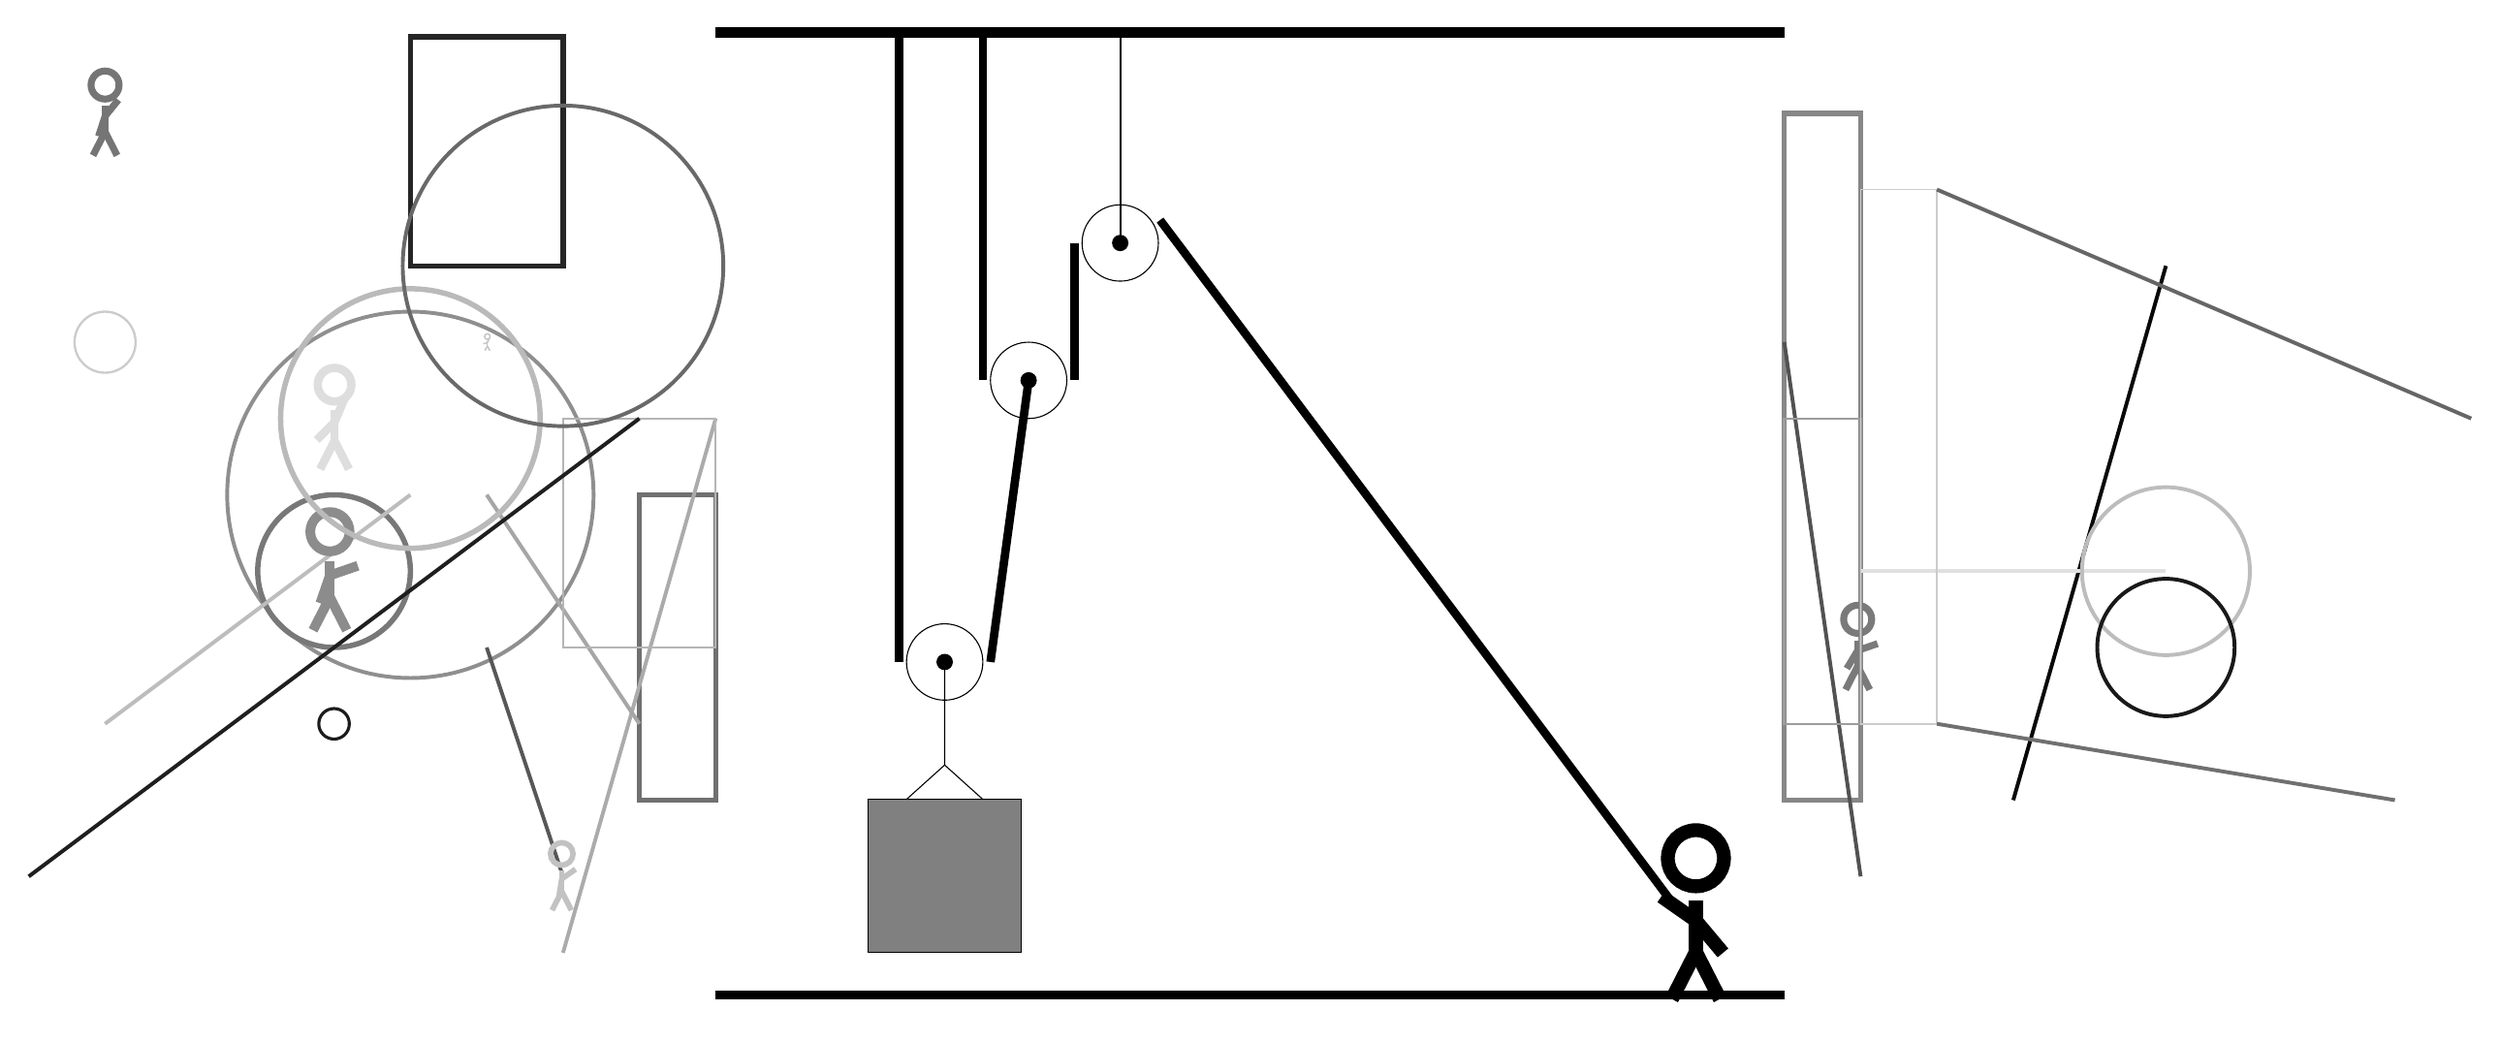
\begin{tikzpicture}
			%%%%% START %%%%%
			
			\draw[fill=black] (-2, 9) rectangle (12, 9.125);
			
			\draw (1, 0.81) circle (0.5);
			\draw[fill=black] (1, 0.81) circle (0.1);
			
			\draw (2.1, 4.5) circle (0.5);
			\draw[fill=black] (2.1, 4.5) circle (0.1);
			
			\draw (3.3, 6.3) circle (0.5);
			\draw[fill=black] (3.3, 6.3) circle (0.1);
			\draw[thick] (3.3, 6.3) -- (3.3, 9);
			
			\draw[line width=0.6mm, color=black!56] (-2, 3) rectangle (-3, -1);
			
			\draw[line width=0.7mm, color=black!47] (12, 8) rectangle (13, -1);
			\draw[line width=0.5mm, color=black!97](17, 6) -- (15, -1);
			\draw [line width=0.5mm, color=black!44](-6, 3) circle (2.4);
			\draw[line width=0.5mm, color=black!68](12, 5) -- (13, -2);
			
			\draw[line width=0.5mm, color=black!66](-4, -2) -- (-5, 1);
			\node[line width=0.2mm, color=black!52] at (13, 1) {\Strichmaxerl[5][59][19]};
			
			\node[line width=0.6mm, color=black!23] at (-5, 5) {\Strichmaxerl[1][12][67]};
			\draw[line width=0.5mm, color=black!33](-2, 4) -- (-4, -3);
			\draw[line width=0.5mm, color=black!35](-3, 0) -- (-5, 3);
			
			\draw[line width=0.3mm, color=black!39] (12, 0) rectangle (13, 4);
			\draw [line width=0.7mm, color=black!53](-7, 2) circle (1.0);
			\draw[line width=0.5mm, color=black!26](-6, 3) -- (-10, 0);
			\draw [line width=0.4mm, color=black!89](-7, 0) circle (0.2);
			\node[line width=0.3mm, color=black!54] at (-10, 8) {\Strichmaxerl[5][72][51]};
			\node[line width=0.5mm, color=black!13] at (-7, 4) {\Strichmaxerl[6][45][67]};
			
			\draw[line width=0.3mm, color=black!29] (-4, 1) rectangle (-2, 4);
			\draw[line width=0.5mm, color=black!12](13, 2) -- (17, 2);
			\draw[line width=0.5mm, color=black!88](-3, 4) -- (-11, -2);
			\draw[line width=0.2mm, color=black!20] (14, 7) rectangle (13, 0);
			\node[line width=0.3mm, color=black!24] at (-4, -2) {\Strichmaxerl[4][81][35]};
			
			\draw [line width=0.3mm, color=black!20](-10, 5) circle (0.4);
			
			\draw[line width=0.5mm, color=black!56](14, 0) -- (20, -1);
			\node[line width=0.4mm, color=black!45] at (-7, 2) {\Strichmaxerl[7][71][19]};
			\draw [line width=0.5mm, color=black!26](17, 2) circle (1.1);
			\draw [line width=0.7mm, color=black!27](-6, 4) circle (1.7);
			\draw[line width=0.7mm, color=black!85] (-4, 9) rectangle (-6, 6);
			\draw [line width=0.5mm, color=black!59](-4, 6) circle (2.1);
			\draw [line width=0.5mm, color=black!90](17, 1) circle (0.9);
			
			\draw[line width=0.5mm, color=black!60](14, 7) -- (21, 4);
			
			\draw (1, 0.81) -- (1, -0.54) -- (0.5, -0.99) -- (1.5, -0.99) -- (1, -0.54);
			\draw[fill=black!50] (0, -0.99) rectangle (2, -2.99);
			
			\draw[line width=1.1mm] (0.4, 9) -- (0.4, 0.81);
			\centerarc[line width=1.1mm](1, 0.81)(180:360:0.6);
			\draw[line width=1.1mm](1.6, 0.81) -- (2.1, 4.5);
			\draw[line width=1.1mm] (1.5, 9) -- (1.5, 4.5);
			\centerarc[line width=1.1mm](2.1, 4.5)(180:360:0.6);
			\draw[line width=1.1mm](2.7, 4.5) -- (2.7, 6.3);
			\centerarc[line width=1.1mm](3.3, 6.3)(30:180:0.6);
			\draw[line width=1.1mm] (3.822, 6.6) -- (10.5, -2.3);
			
			\node at (10.8, -2.5) {\Strichmaxerl[10][-35][-50]};
			
			\draw[fill=black] (-2, -3.5) rectangle (12, -3.6);
			
			%%%%% END %%%%%
		\end{tikzpicture}
	\end{figure}	
\end{document}